\documentclass[table]{beamer}
\usepackage{graphicx}
\usepackage{color}
\usepackage{pgfpages}
\usepackage{amsmath}
\usepackage{booktabs}
\usepackage{listings}
\usepackage{graphicx}
\usepackage{multirow}

\makeatother
\setbeamertemplate{footline}
{
  % \leavevmode%
  % \hbox{%
  % \begin{beamercolorbox}[wd=.4\paperwidth,ht=2.25ex,dp=1ex,center]{author in head/foot}%
  %   \usebeamerfont{author in head/foot}\insertshortauthor
  % \end{beamercolorbox}%
  % \begin{beamercolorbox}[wd=.6\paperwidth,ht=2.25ex,dp=1ex,center]{title in head/foot}%
  %   \usebeamerfont{title in head/foot}\insertshorttitle\hspace*{3em}
  %   \insertframenumber{} / \inserttotalframenumber\hspace*{1ex}
  % \end{beamercolorbox}}%
  % \vskip0pt%
}
\makeatletter

\setbeamertemplate{footline}[page number]{}

\setbeamertemplate{navigation symbols}{}

\definecolor{mygray}{rgb}{0.9,0.9,0.9}

\lstset{
    basicstyle=\footnotesize\ttfamily,
    tabsize=2,
    backgroundcolor=\color{mygray},
    escapeinside={(*}{*)}
}

\usetheme{Szeged} 
\usecolortheme{beaver}

% Remove nav buttons
% \beamertemplatenavigationsymbolsempty
\setbeamercolor{navigation symbols}{fg=black, bg=white}



\title{Safety $\neq$ Security}
\subtitle{A SECURITY EVALUATION OF STATE OF THE ART AUTOMOTIVE MICROCONTROLLERS}
\date{May 10, 2017}
\author{Nils Wiersma}

\titlegraphic{\includegraphics[width=3cm]{../../pics/riscurelogo.png}% \hspace{5cm}% \ \\%
  \hspace{1cm}  
 \includegraphics[width=5cm]{../../pics/rulogo.pdf}
}


\usepackage{cleveref}

\usepackage{import}
\graphicspath{{pics/}{../../pics/}}

\begin{document}

\begin{frame}
    \titlepage
\end{frame}

\begin{frame}
    \tableofcontents
\end{frame}

\section{Introduction}

\begin{frame}
    \tableofcontents[currentsection]
\end{frame}


\begin{frame}{Topic}
    \begin{itemize}
        \item[] Investigate the security of modern microcontroller units, 
            \item[] used in the automotive industry, 
            \item[] by means of fault injection.
    \end{itemize}
\end{frame}

\begin{frame}{Why the automotive microcontrollers?}
    
    \begin{itemize}
        \item Safety critical
        \item Fault tolerance
        \item ISO26262
        \item Safety mechanisms $\rightarrow$ countermeasures
    \end{itemize}
\end{frame}

\begin{frame}{Safety mechanisms / Countermeasures}{Duplicate execution and compare (lockstep)}
    \begin{figure}[H]
      \centering
      \def\svgwidth{\columnwidth}
      \input{../../pics/lockstepdiagram.pdf_tex}
      \label{fig:lockstepdiagram}
    \end{figure}
\end{frame}

\begin{frame}{Safety mechanisms / Countermeasures}{Memory}
    \begin{itemize}
        \item Error correction and detection codes
        \item Memory duplication
    \end{itemize}
\end{frame}


\section{Setup}

\begin{frame}
    \tableofcontents[currentsection]
\end{frame}

\begin{frame}{Techniques}
    \begin{itemize}
        \item Power
        \item Electromagnetic
    \end{itemize}
\end{frame}

\begin{frame}{Setup}
    \begin{figure}[H]
    \centering
    \def\svgwidth{\columnwidth}
    \input{../../pics/FIdiagram-icWaves.pdf_tex}
    \end{figure}
\end{frame}

% \begin{frame}{Setup}
%     \begin{figure}[H]
%     \centering
%     \def\svgwidth{\columnwidth}
%     \input{../../pics/FIdiagram-EM.pdf_tex}
%     \end{figure}
% \end{frame}


\section{Targets}
\begin{frame}
    \tableofcontents[currentsection]
\end{frame}

\begin{frame}[t]{Targets}
    \begin{figure}[H]
      \centering
      \includegraphics[width=.6\textwidth]{../../pics/spc570-cutout.png}
      % \caption{\TI \unroll glitch offset vs. length}
      % \label{fig:ti-unroll-offset-length}
    \end{figure}

    \begin{itemize}
        \item e200z0h PowerPC 32bit by STMicroelectronics  
    \end{itemize}
\end{frame}

\begin{frame}[t]{Targets}
    \begin{figure}[H]
      \centering
      \includegraphics[width=.7\textwidth]{../../pics/tms570-cutout.png}
      % \caption{\TI \unroll glitch offset vs. length}
      % \label{fig:ti-unroll-offset-length}
    \end{figure}

    \begin{itemize}
        \item Cortex-R4F ARM 32bit by Texas Instruments
    \end{itemize}
\end{frame}

\begin{frame}[t]{Targets}
    \begin{figure}[H]
      \centering
      \includegraphics[width=.7\textwidth]{../../pics/xpr_lpc1114.png}
      % \caption{\TI \unroll glitch offset vs. length}
      % \label{fig:ti-unroll-offset-length}
    \end{figure}

    \begin{itemize}
        \item Cortex-M0 ARM 32bit by NXP (no fancy countermeasures)
    \end{itemize}
\end{frame}

\begin{frame}{Targets}

      \begin{table}[H]
            \centering
        \begin{tabular}{rcccccc}
        % \toprule
        Assurance level && Low &  \multicolumn{3}{c}{$\xrightarrow{\hspace*{3cm}}$}      & High \\
                        % & &&&&\\
                         &\multicolumn{3}{l}{\includegraphics[width=.2\textwidth]{../../pics/xpr_lpc1114.png}} &&\multicolumn{2}{r}{\includegraphics[width=.2\textwidth]{../../pics/tms570+spc570.png}} \\
                        % & &&&&\\
        Category        && QM  & ASIL-A & ASIL-B & ASIL-C & ASIL-D \\
        % \cmidrule{1-6}
        % \bottomrule
        \end{tabular}
        % \caption{ASIL categories} 
        % \label{tab:ASIL}
      \end{table}

\end{frame}

\section{Characterization}
\begin{frame}
    \tableofcontents[currentsection]
\end{frame}


\begin{frame}{Experiments}
    \begin{itemize}
        \item Characterization of targets
        \item Unlocking debug interface (JTAG)
    \end{itemize}
\end{frame}

\begin{frame}{Characterization}
    \begin{itemize}
        \item[] Target firmware under complete control of the attacker
    \end{itemize}
    \begin{itemize}
      \item[] Nice trigger signals
      \begin{itemize}
        \item reduce variables to minimum
      \end{itemize} 
      \item[] Nice output
      \begin{itemize}
        \item classify attempts
        \item investigate state after fault
      \end{itemize} 
    \end{itemize}

    
\end{frame}

% \begin{frame}{Characterization}
%     \begin{itemize}
%         \item Experiment 1: unrolled loop of add instructions
%         \begin{itemize}
%             \item[] explore sensitivity and broad parameters
%         \end{itemize}
%         \item Experiment 2: simple authentication check
%         \begin{itemize}
%             \item[] a more realistic setting
%         \end{itemize}
%     \end{itemize}
% \end{frame}

\begin{frame}{Characterization}{Experiment 1: unrolled loop of add instructions}
    trigger\_high() \\
    \ \\
    ADD r1 \#1 \\
    ADD r1 \#1 \\
    ADD r1 \#1 \\
    ADD r1 \#1 \\
    ADD r1 \#1 \\
    ADD r1 \#1 \\
    \ \\
    trigger\_low() \\
    serial\_send(r1) \\
    % \begin{itemize}
    %     \item Investigate value after execution, deviation from expected value means successful fault
    % \end{itemize}
\end{frame}

\begin{frame}{Characterization}{Experiment 2: simple authentication check}

    flag = 1 \\
    trigger\_high() \\
    \ \\
    if (flag == 0): \\
    \     authenticated() \\
    else: \\
    \     not\_authenticated() \\
    \ \\
    trigger\_low() \\
\end{frame}

\begin{frame}{Characterization}
    \begin{enumerate}
        \item Investigate normal behavior through (side) channels 
        \item Determine rough ranges of values for different parameters
        \item Determine fixed values for parameters that yield good results
    \end{enumerate}
\end{frame}

\begin{frame}{Characterization}
    \begin{enumerate}
        \item Investigate normal behavior through (side) channels 
        \item Determine rough ranges of values for different parameters
        \item \textbf{Determine fixed values for parameters that yield good results}
    \end{enumerate}
\end{frame}

% \begin{frame}{Characterization}{1. Investigate normal behavior through (side) channels \\ 2. Determine rough ranges of values for different parameters}

%     \begin{figure}[H]
%     \centering
%     \def\svgwidth{\columnwidth}
%     \input{../../pics/FIdiagram-icWaves.pdf_tex}
%     \end{figure}

% \end{frame}
\begin{frame}{Characterization}{TI Power ADD voltage vs. offset}
    \vspace{-.3cm}
    \begin{figure}[H]
      \centering
      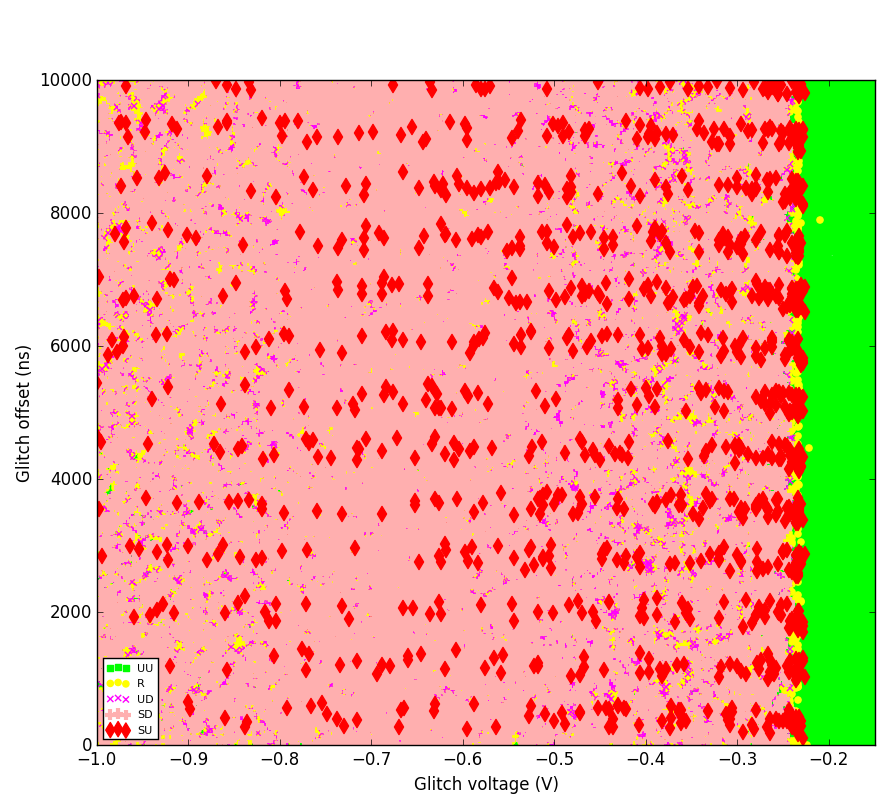
\includegraphics[width=.7\textwidth]{../../plots/newplots/ti-add-voltage-offset.png}
    \end{figure}
\end{frame}

\begin{frame}{Characterization}{TI Power ADD voltage vs. length}
    \vspace{-.3cm}
    \begin{figure}[H]
      \centering
      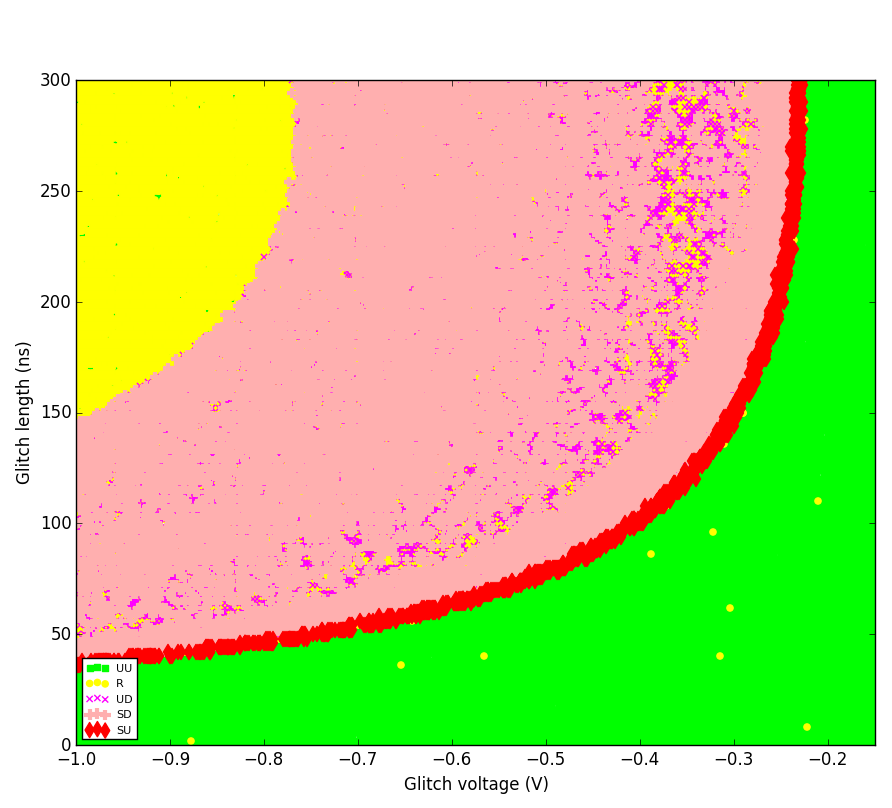
\includegraphics[width=.7\textwidth]{../../plots/newplots/ti-add-voltage-length.png}
    \end{figure}
\end{frame}

\begin{frame}{Characterization}{TI Power BRANCH offset vs. length}
    \vspace{-.3cm}
    \begin{figure}[H]
      \centering
      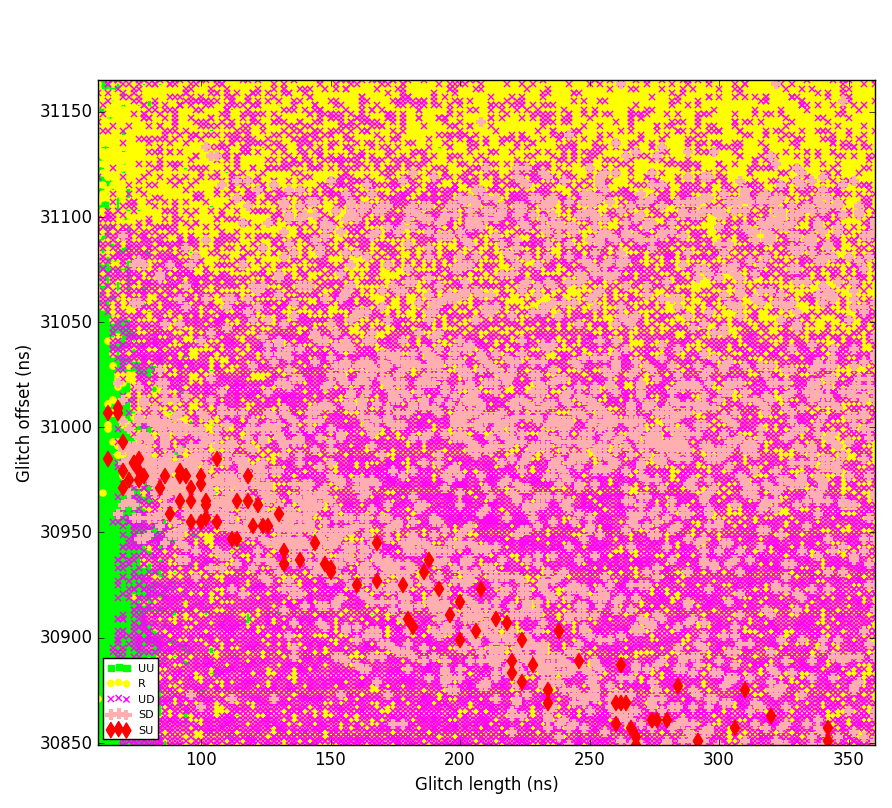
\includegraphics[width=.7\textwidth]{../../plots/newplots/ti-auth-length-offset.png}
    \end{figure}
\end{frame}

\begin{frame}{Characterization}{TI Power BRANCH offset vs. voltage}
    \vspace{-.3cm}
    \begin{figure}[H]
      \centering
      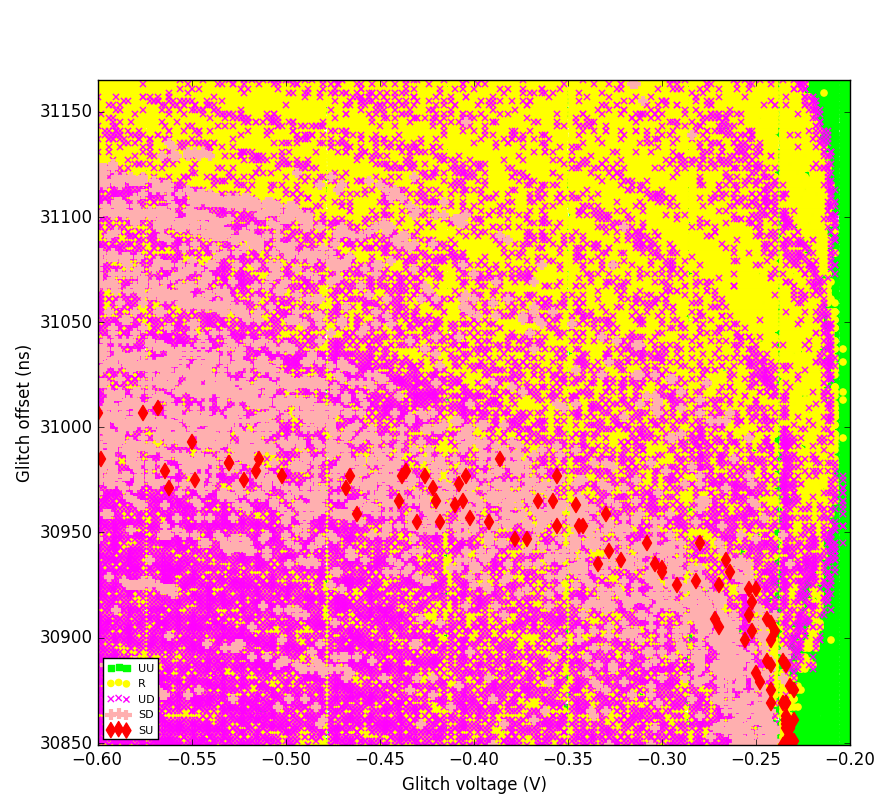
\includegraphics[width=.7\textwidth]{../../plots/newplots/ti-auth-voltage-offset.png}
    \end{figure}
\end{frame}

\begin{frame}{Characterization}{TI Power BRANCH length vs. voltage}
    \vspace{-.3cm}
    \begin{figure}[H]
      \centering
      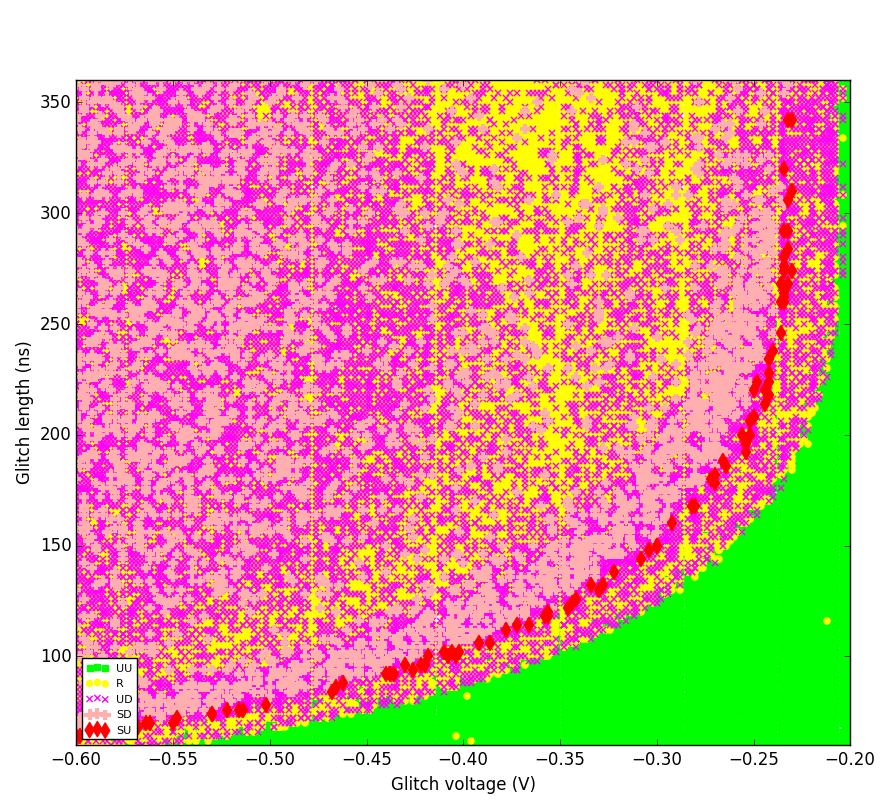
\includegraphics[width=.7\textwidth]{../../plots/newplots/ti-auth-voltage-length.png}
    \end{figure}
\end{frame}

\begin{frame}{Characterization}{TI Power BRANCH length vs. voltage, offset binned (40ns) 1/4}
    \vspace{-.3cm}
    \begin{figure}[H]
      \centering
      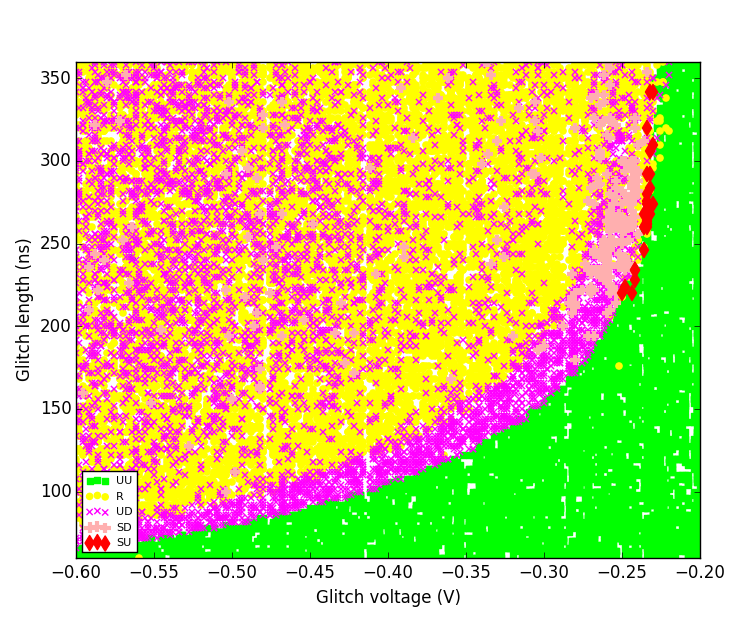
\includegraphics[width=.75\textwidth]{../../plots/newplots/ti-auth-voltage-length-offets-1.png}
    \end{figure}
\end{frame}
\begin{frame}{Characterization}{TI Power BRANCH length vs. voltage, offset binned (40ns) 2/4}
    \vspace{-.3cm}
    \begin{figure}[H]
      \centering
      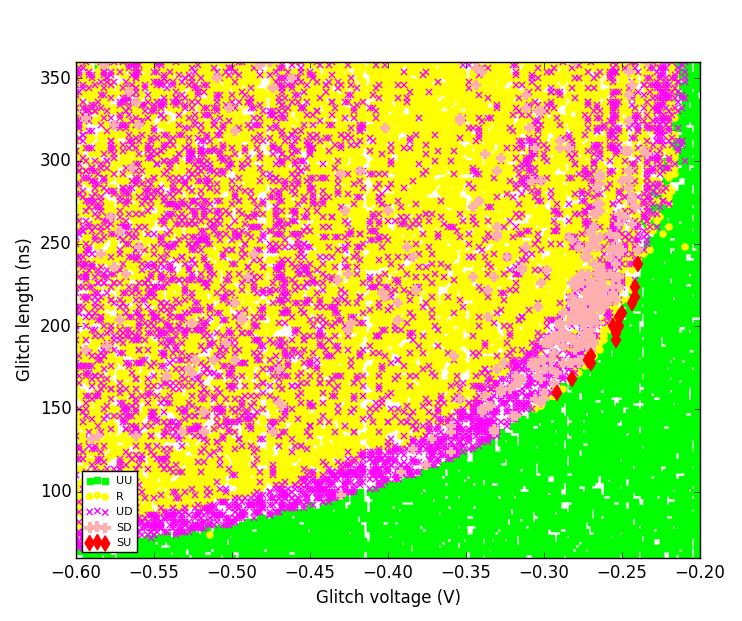
\includegraphics[width=.75\textwidth]{../../plots/newplots/ti-auth-voltage-length-offets-2.png}
    \end{figure}
\end{frame}
\begin{frame}{Characterization}{TI Power BRANCH length vs. voltage, offset binned (40ns) 3/4}
    \vspace{-.3cm}
    \begin{figure}[H]
      \centering
      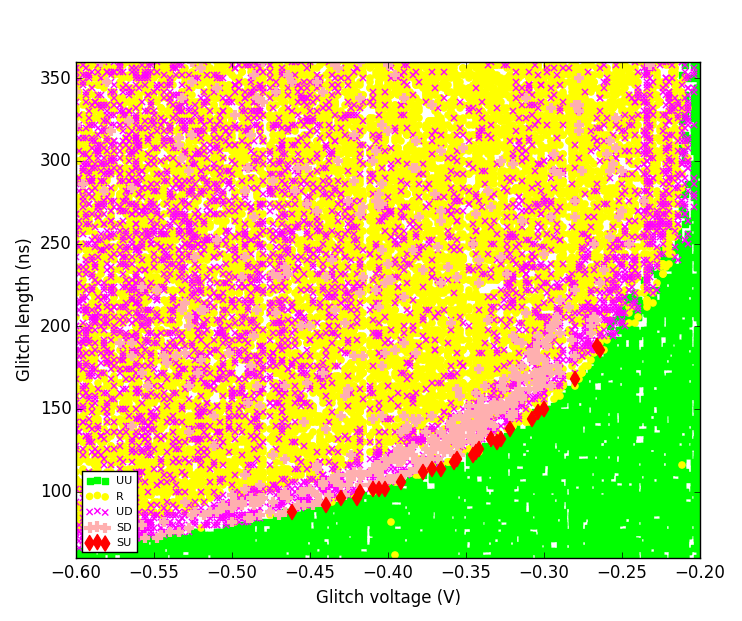
\includegraphics[width=.75\textwidth]{../../plots/newplots/ti-auth-voltage-length-offets-3.png}
    \end{figure}
\end{frame}
\begin{frame}{Characterization}{TI Power BRANCH length vs. voltage, offset binned (40ns) 4/4}
    \vspace{-.3cm}
    \begin{figure}[H]
      \centering
      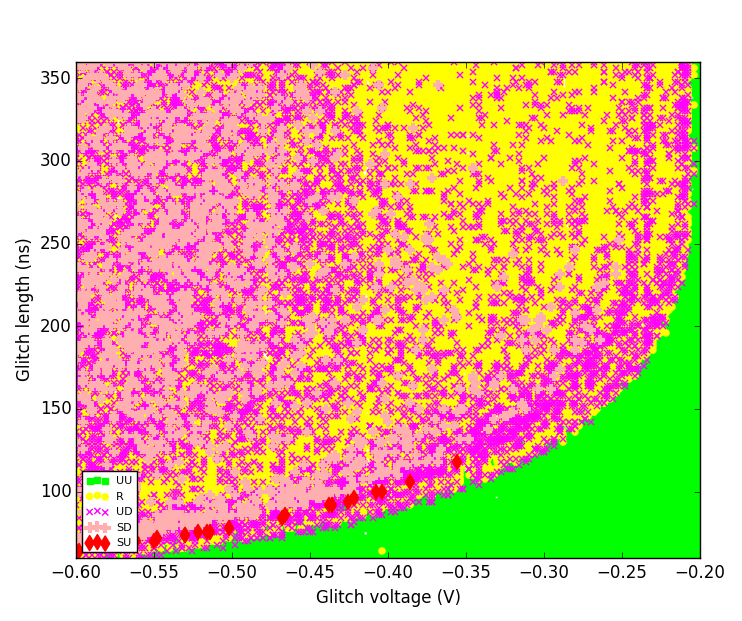
\includegraphics[width=.75\textwidth]{../../plots/newplots/ti-auth-voltage-length-offets-4.png}
    \end{figure}
\end{frame}

\begin{frame}{Characterization}{Length vs. voltage vs. offset}
    \vspace{-.3cm}
    \begin{figure}[H]
      \centering
      \includegraphics[width=.8\textwidth]{../../pics/slope-diagram.png}
    \end{figure}
\end{frame}

\begin{frame}{Characterization}{ST EM ADD X,Y position, glitch power binned (20\%) 1/4}
    \vspace{-.3cm}
    \begin{figure}[H]
      \centering
      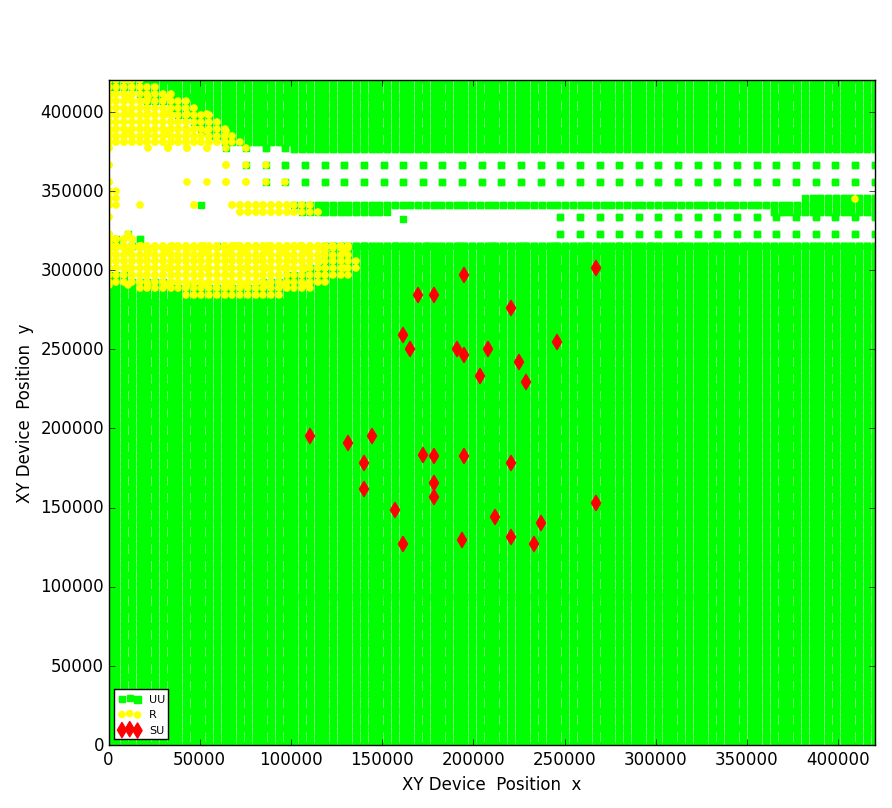
\includegraphics[width=.75\textwidth]{../../plots/newplots/st-add-x-y-power-1.png}
    \end{figure}
\end{frame}
\begin{frame}{Characterization}{ST EM ADD X,Y position, glitch power binned (20\%) 2/4}
    \vspace{-.3cm}
    \begin{figure}[H]
      \centering
      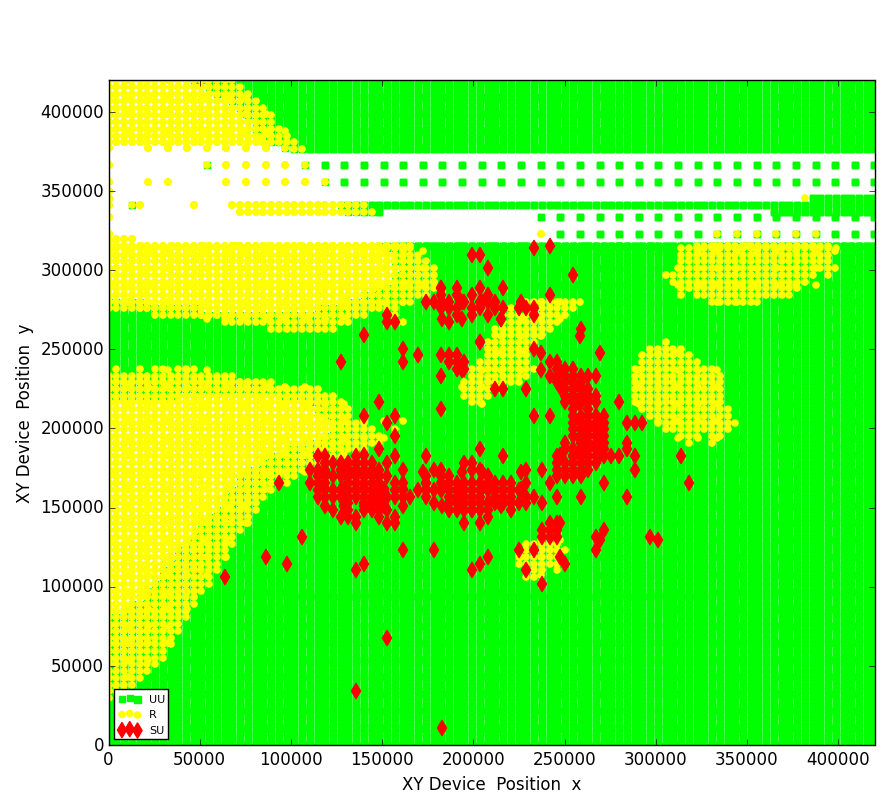
\includegraphics[width=.75\textwidth]{../../plots/newplots/st-add-x-y-power-2.png}
    \end{figure}
\end{frame}
\begin{frame}{Characterization}{ST EM ADD X,Y position, glitch power binned (20\%) 3/4}
    \vspace{-.3cm}
    \begin{figure}[H]
      \centering
      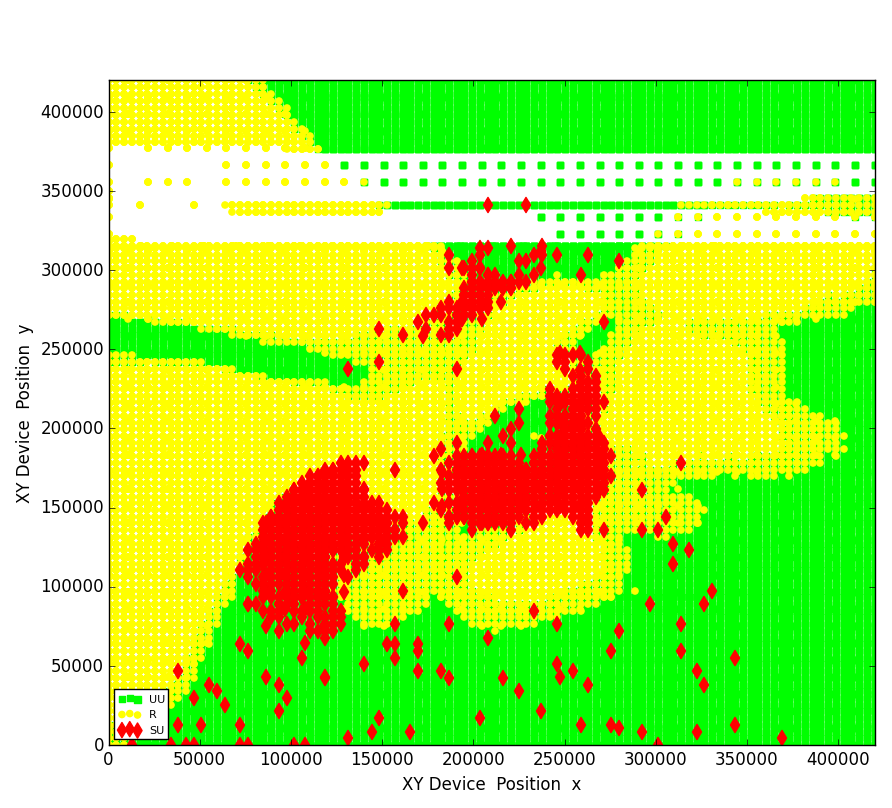
\includegraphics[width=.75\textwidth]{../../plots/newplots/st-add-x-y-power-3.png}
    \end{figure}
\end{frame}
\begin{frame}{Characterization}{ST EM ADD X,Y position, glitch power binned (20\%) 4/4}
    \vspace{-.3cm}
    \begin{figure}[H]
      \centering
      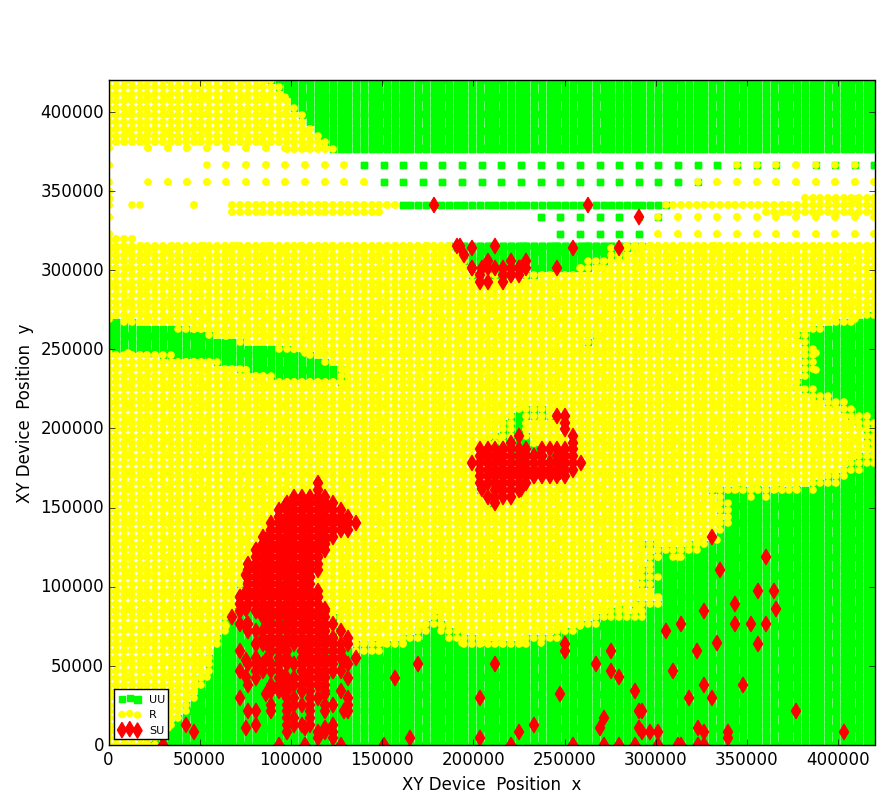
\includegraphics[width=.75\textwidth]{../../plots/newplots/st-add-x-y-power-4.png}
    \end{figure}
\end{frame}

\begin{frame}{Characterization}{TI EM BRANCH X,Y position on die}
    \vspace{-.3cm}
    \begin{figure}[H]
      \centering
      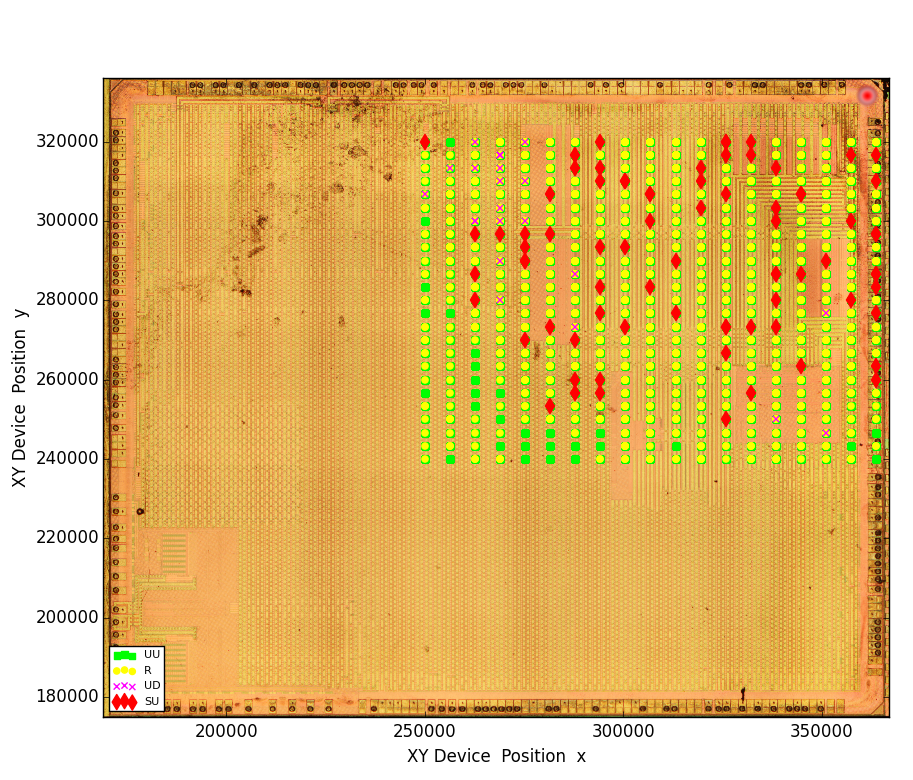
\includegraphics[width=.75\textwidth]{../../plots/newplots/ti-auth-x-y-ondie.png}
    \end{figure}
\end{frame}

\begin{frame}{Characterization}{3. Determine fixed values for parameters that yield good results}
    \vspace{-.3cm}
    MORE  PLOTSSS
\ \\
% 260 000 measurements
\end{frame}


\begin{frame}{Characterization}{Branch experiment results summary}{Power}
    \begin{table}[H]
          \centering
          \begin{tabular}{c c c}
          \toprule
            \cellcolor{white!100} Target & Successful & Detected \\
            \midrule
            \includegraphics[width=.2\textwidth]{../../pics/tms570-cutout.png} & \multirow{ 2}{*}{60\%} & \multirow{ 2}{*}{0\%} \\ TI & &\\
            \cmidrule{1-3}
            \includegraphics[width=.2\textwidth]{../../pics/spc570-cutout.png} & \multirow{ 2}{*}{0\%$^*$} & \multirow{ 2}{*}{0\%$^*$} \\ STM& &\\
          \bottomrule
          \end{tabular}
    \end{table}
\end{frame}

\begin{frame}{Characterization}{Branch experiment results summary}{EM}
    \begin{table}[H]
          \centering
          \begin{tabular}{c c c}
          \toprule
            \cellcolor{white!100} Target & Successful & Detected \\
            \midrule
            \includegraphics[width=.2\textwidth]{../../pics/tms570-cutout.png} & \multirow{ 2}{*}{0.2\%$^*$} & \multirow{ 2}{*}{0.07\%$^*$} \\ TI & &\\
            \cmidrule{1-3}
            \includegraphics[width=.2\textwidth]{../../pics/spc570-cutout.png} & \multirow{ 2}{*}{58\%} & \multirow{ 2}{*}{0\%$^*$} \\ STM& &\\
          \bottomrule
          \end{tabular}
    \end{table}
\end{frame}

\begin{frame}{Characterization}{ Comparison of triggered measures in TI}
    % \begin{itemize}
    %     \item Comparison of triggered measures in TI
    % \end{itemize}
    
    \begin{table}[H]
          \centering
          \begin{tabular}{r r r}
          \toprule
            Successful & Detected & Other \\
            \midrule
            % Experiment 1 (ADD) & 0.7\% & 25\% & 74\% \\
            % Experiment 2 (CHECK) & 
            0.7\% & 24\% & 75\% \\
          \bottomrule
          \end{tabular}
    \end{table}

    \begin{table}[H]
          \centering
          \begin{tabular}{ r r r}
          \toprule
             Lockstep & RAM parity & Flash address parity \\
            \midrule
            % ADD & 92\% & 26\% & 12\% \\
            % CHECK &
             98\% & 21\% & 27\% \\
          \bottomrule
          \end{tabular}
    \end{table}

    % \begin{itemize}
    %     \item Most effective: lockstep
    % \end{itemize}
\end{frame}

\section{JTAG}
\begin{frame}
    \tableofcontents[currentsection]
\end{frame}

\begin{frame}{JTAG}
    \begin{itemize}
        \item Locked, unlockable by providing password
        \item No knowledge of firmware
        \item No clear trigger signals available
        \item No register output to categorize
    \end{itemize}

    \begin{itemize}
      \item Read memory
      \begin{itemize}
        \item Asset by itself
        \item Stepping stone to other assets
      \end{itemize}
    \end{itemize}
\end{frame}

\begin{frame}{JTAG}
    \begin{figure}[H]
      \centering
      \includegraphics[width=.7\textwidth]{../../pics/tms570-cutout.png}
      % \caption{\TI \unroll glitch offset vs. length}
      % \label{fig:ti-unroll-offset-length}
    \end{figure}
\end{frame}

\begin{frame}{JTAG}
  \begin{itemize}
    \item JTAG password in memory
    \item JTAG locking during boot sequence
  \end{itemize}
    \begin{itemize}
        \item Differential analysis of locked and unlocked target
        \item Inject fault during boot
        \item Obtain JTAG password for persistent access
    \end{itemize}
\end{frame}

\begin{frame}{JTAG}
    \begin{enumerate}
        \item Investigate normal behavior through (side) channels 
        \item Determine rough ranges of values for different parameters
        \item Determine fixed values for parameters that yield good results
    \end{enumerate}
\end{frame}


\begin{frame}{JTAG}
    \begin{enumerate}
        \item \textbf{Investigate normal behavior through (side) channels} 
        \item Determine rough ranges of values for different parameters
        \item Determine fixed values for parameters that yield good results
    \end{enumerate}

    \ \\
    (thank you Fatih!)
\end{frame}


\begin{frame}{JTAG}{1. Investigate normal behavior through (side) channels }
    \begin{figure}[H]
      \centering
      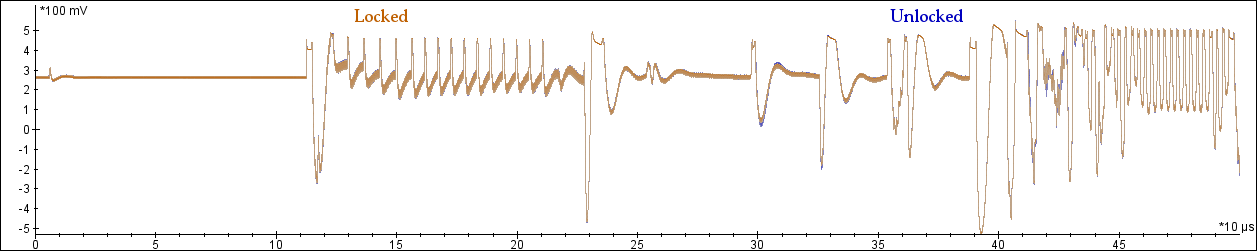
\includegraphics[width=\textwidth]{../plots/tms57-trace1.png}
    \end{figure}
\end{frame}

\begin{frame}{JTAG}{1. Investigate normal behavior through (side) channels }
    \begin{figure}[H]
      \centering
      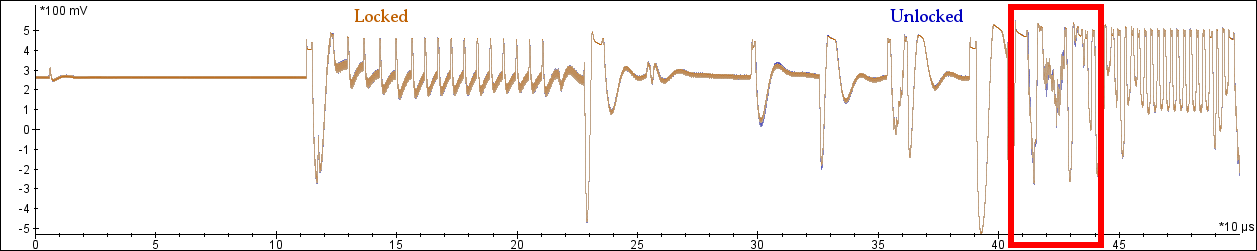
\includegraphics[width=\textwidth]{../plots/tms57-trace1-2.png}
    \end{figure}
\end{frame}

\begin{frame}{JTAG}{1. Investigate normal behavior through (side) channels }
    \begin{figure}[H]
      \centering
      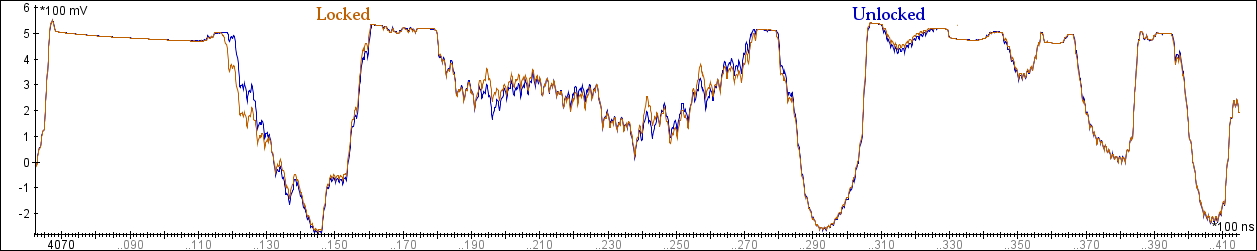
\includegraphics[width=\textwidth]{../plots/tms57-trace2.png}
    \end{figure}
\end{frame}

\begin{frame}{JTAG}{1. Investigate normal behavior through (side) channels }
    \begin{figure}[H]
      \centering
      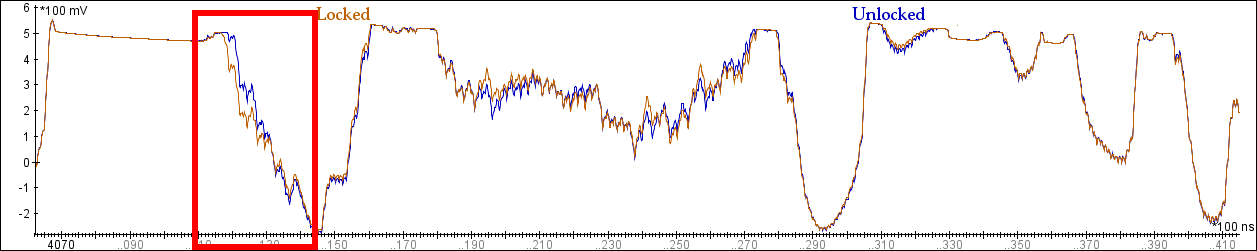
\includegraphics[width=\textwidth]{../plots/tms57-trace2-2.png}
    \end{figure}
\end{frame}


\begin{frame}{JTAG}
    \begin{enumerate}
        \item Investigate normal behavior through (side) channels 
        \item Determine rough ranges of values for different parameters
        \item \textbf{Determine fixed values for parameters that yield good results}
    \end{enumerate}
\end{frame}

\begin{frame}{JTAG}{TI power JTAG offset vs. voltage}
    \vspace{-.3cm}
    \begin{figure}[H]
      \centering
      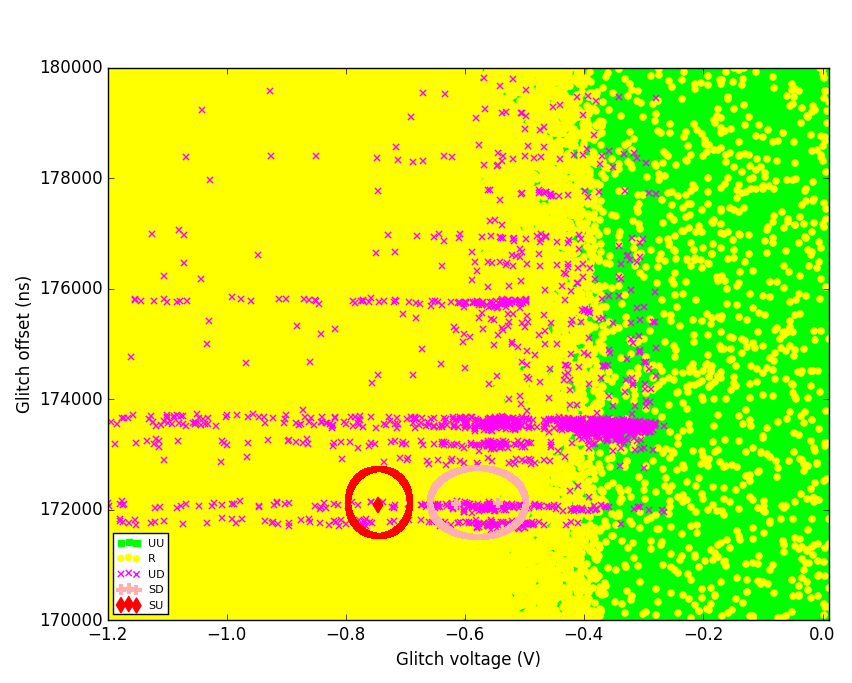
\includegraphics[width=.8\textwidth]{../../plots/newplots/ti-jtag-voltage-offset.png}
    \end{figure}
% 260 000 measurements
\end{frame}

\begin{frame}{JTAG}{TI power JTAG length vs. voltage}
    \vspace{-.3cm}
    \begin{figure}[H]
      \centering
      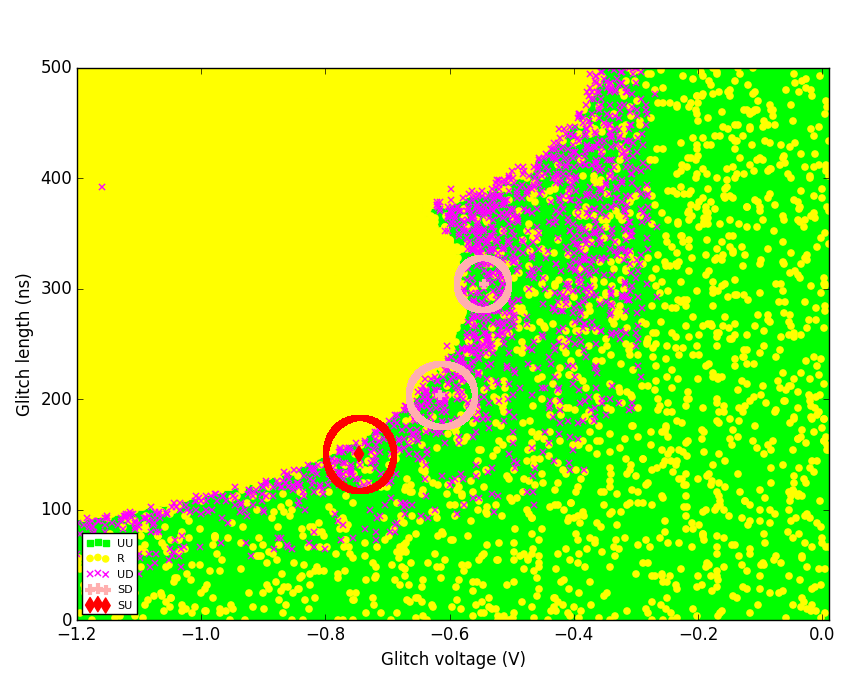
\includegraphics[width=.8\textwidth]{../../plots/newplots/ti-jtag-voltage-length.png}
    \end{figure}
% 260 000 measurements
\end{frame}

\begin{frame}{JTAG}
    \begin{table}[H]
          \centering
          \begin{tabular}{c c c}
          \toprule
            \cellcolor{white!100} Target & Successful & Detected \\
            \midrule
            \includegraphics[width=.2\textwidth]{../../pics/tms570-cutout.png} & \multirow{ 2}{*}{1.4\%} & \multirow{ 2}{*}{4.5\%} \\ TI (power) & &\\
            % \cmidrule{1-3}
            % \includegraphics[width=.2\textwidth]{../../pics/spc570-cutout.png} & \multirow{ 2}{*}{58\%} & \multirow{ 2}{*}{0\%} \\ STM (EM) & &\\
          \bottomrule
          \end{tabular}
    \end{table}
\end{frame}

\begin{frame}{JTAG}
    \begin{figure}[H]
      \centering
      \includegraphics[width=.7\textwidth]{../../pics/xpr_lpc1114.png}
      % \caption{\TI \unroll glitch offset vs. length}
      % \label{fig:ti-unroll-offset-length}
    \end{figure}

    (done by Ramiro)
\end{frame}

\begin{frame}{JTAG}
  % \begin{itemize}
    % \item JTAG p/assword in memory
    % \item JTAG locking during boot sequence
  % \end{itemize}
    \begin{itemize}
        \item Correlation analysis by repeatedly changing bits in the password
        % \item Inject fault during boot
        % \item Obtain JTAG password for persistent access
    \end{itemize}
\end{frame}

% \begin{frame}{JTAG}
%     \begin{enumerate}
%         \item Investigate normal behavior through (side) channels 
%         \item Determine rough ranges of values for different parameters
%         \item Determine fixed values for parameters that yield good results
%     \end{enumerate}
% \end{frame}


% \begin{frame}{JTAG}
%     \begin{enumerate}
%         \item \textbf{Investigate normal behavior through (side) channels} 
%         \item Determine rough ranges of values for different parameters
%         \item Determine fixed values for parameters that yield good results
%     \end{enumerate}

%     \ \\
%     (thank you Fatih!)
% \end{frame}


\begin{frame}{JTAG}{1. Investigate normal behavior through (side) channels }
    \begin{figure}[H]
      \centering
      \includegraphics[width=\textwidth]{../pics/lpc-corr.png}
    \end{figure}
\end{frame}

\begin{frame}{JTAG}{1. Investigate normal behavior through (side) channels }
    \begin{figure}[H]
      \centering
      \includegraphics[width=\textwidth]{../pics/lpc-corr-zoom.png}
    \end{figure}
\end{frame}

\begin{frame}{JTAG}{NXP power JTAG offset vs. voltage}
    \vspace{-.3cm}
    \begin{figure}[H]
      \centering
      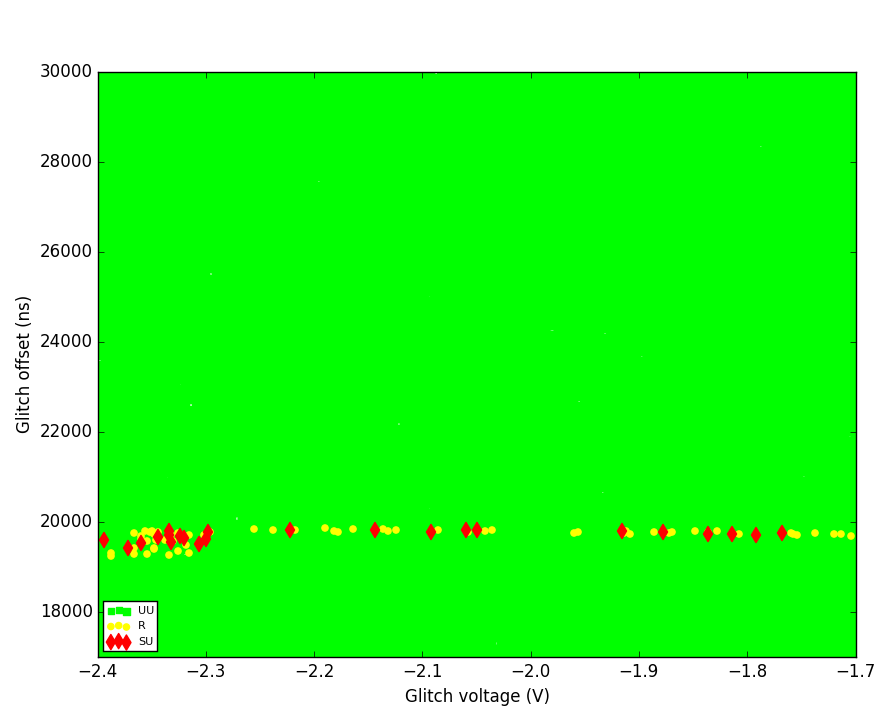
\includegraphics[width=.8\textwidth]{../../plots/newplots/nxp-jtag-voltage-offset.png}
    \end{figure}
\end{frame}

\begin{frame}{JTAG}{NXP power JTAG offset vs. voltage}
    \vspace{-.3cm}
    \begin{figure}[H]
      \centering
      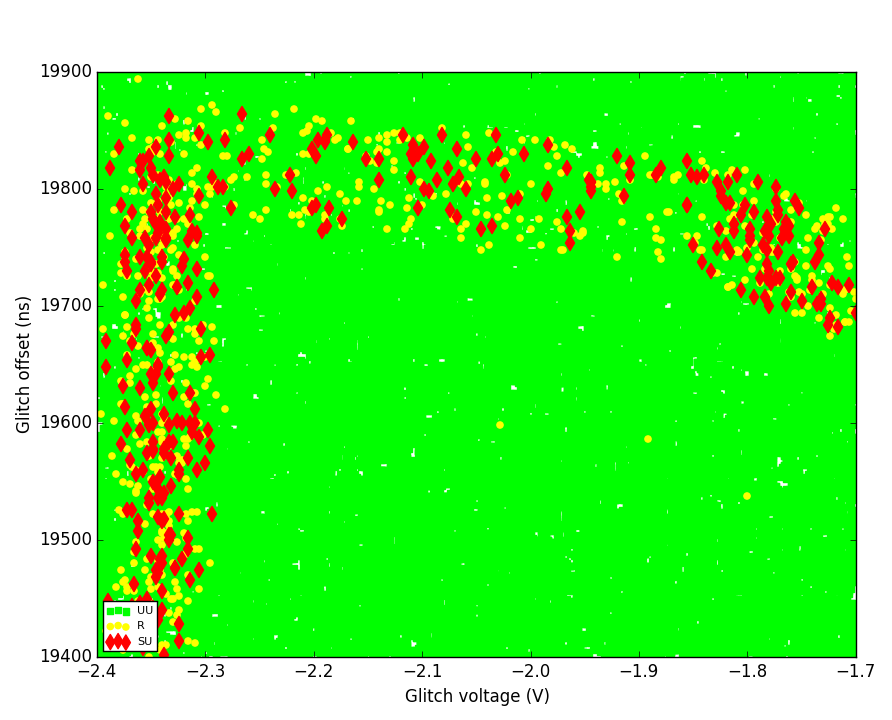
\includegraphics[width=.8\textwidth]{../../plots/newplots/nxp-jtag-voltage-offset-2.png}
    \end{figure}
\end{frame}

\begin{frame}{JTAG}{NXP power JTAG length vs. voltage}
    \vspace{-.3cm}
    \begin{figure}[H]
      \centering
      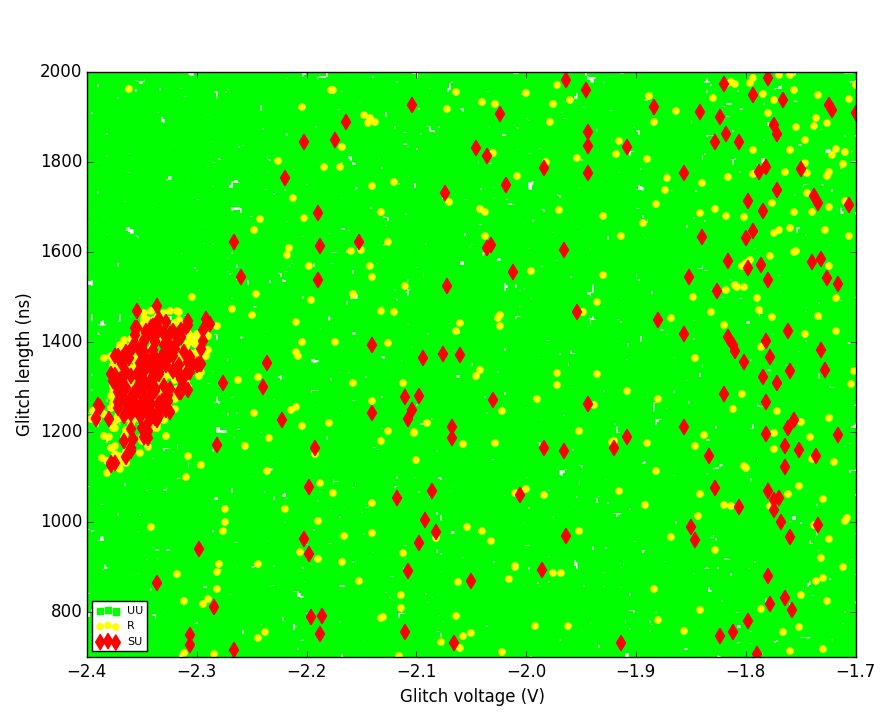
\includegraphics[width=.8\textwidth]{../../plots/newplots/nxp-jtag-voltage-length.png}
    \end{figure}
\end{frame}

\begin{frame}{JTAG}{NXP power JTAG length vs. voltage, binned offset (125ns) 1/4}
    \vspace{-.3cm}
    \begin{figure}[H]
      \centering
      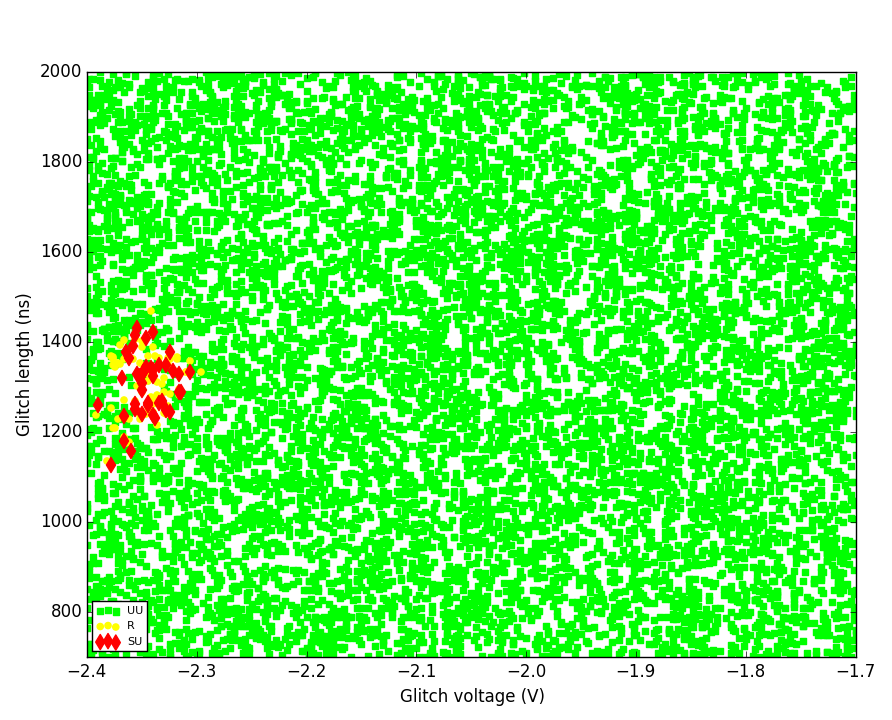
\includegraphics[width=.8\textwidth]{../../plots/newplots/nxp-jtag-voltage-length-1.png}
    \end{figure}
\end{frame}
\begin{frame}{JTAG}{NXP power JTAG length vs. voltage, binned offset (125ns) 2/4}
    \vspace{-.3cm}
    \begin{figure}[H]
      \centering
      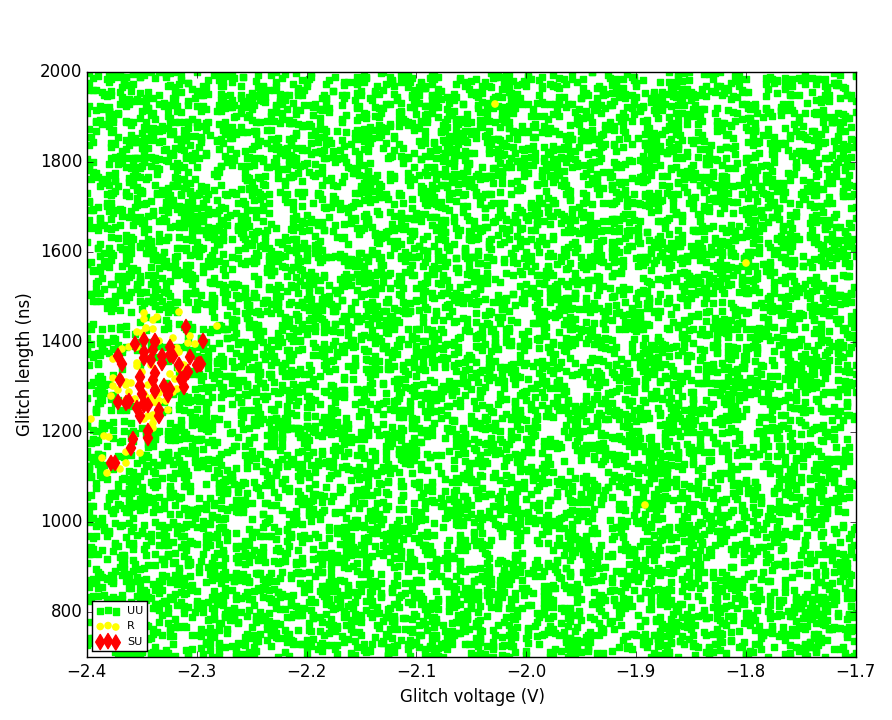
\includegraphics[width=.8\textwidth]{../../plots/newplots/nxp-jtag-voltage-length-2.png}
    \end{figure}
\end{frame}
\begin{frame}{JTAG}{NXP power JTAG length vs. voltage, binned offset (125ns) 3/4}
    \vspace{-.3cm}
    \begin{figure}[H]
      \centering
      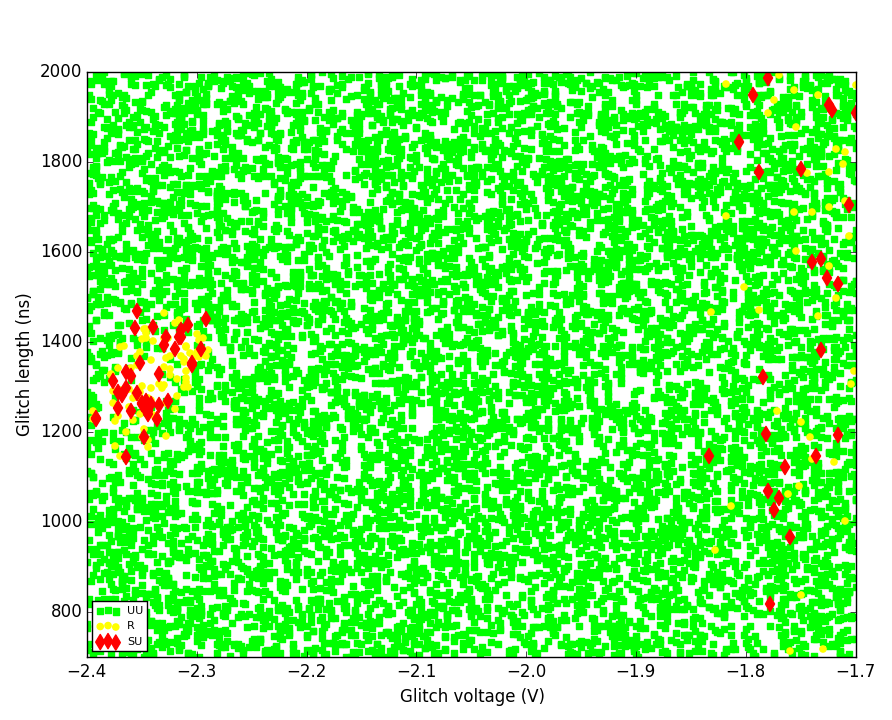
\includegraphics[width=.8\textwidth]{../../plots/newplots/nxp-jtag-voltage-length-3.png}
    \end{figure}
\end{frame}
\begin{frame}{JTAG}{NXP power JTAG length vs. voltage, binned offset (125ns) 4/4}
    \vspace{-.3cm}
    \begin{figure}[H]
      \centering
      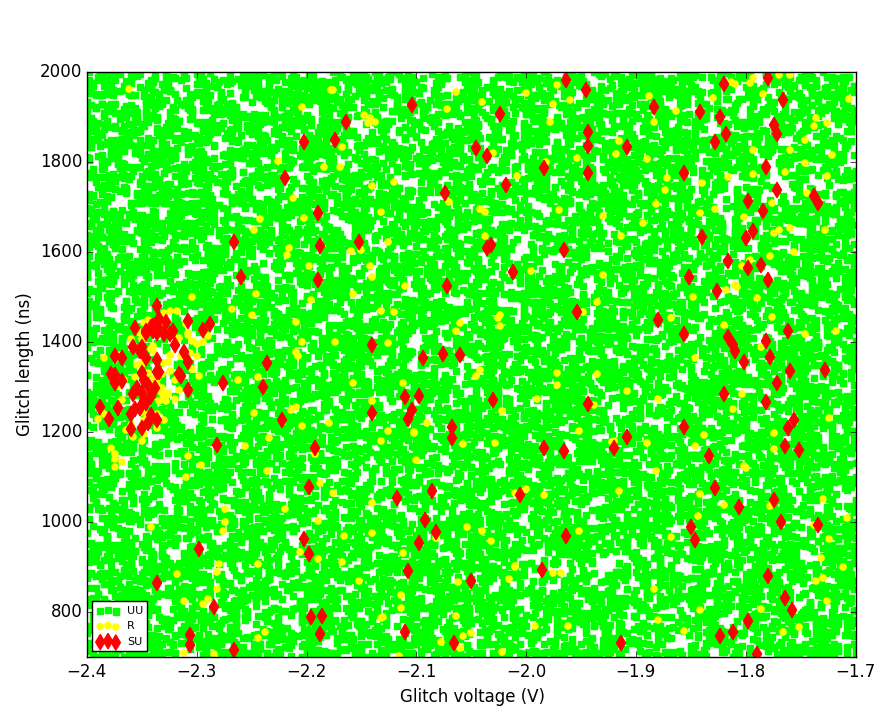
\includegraphics[width=.8\textwidth]{../../plots/newplots/nxp-jtag-voltage-length-4.png}
    \end{figure}
\end{frame}

\begin{frame}{JTAG}
    \begin{table}[H]
          \centering
          \begin{tabular}{c c c}
          \toprule
            \cellcolor{white!100} Target & Successful & Detected \\
            \midrule
            \includegraphics[width=.2\textwidth]{../../pics/tms570-cutout.png} & \multirow{ 2}{*}{1.4\%} & \multirow{ 2}{*}{4.5\%} \\ TI (power) & &\\
            \cmidrule{1-3}
            \includegraphics[width=.2\textwidth]{../../pics/xpr_lpc1114.png} & \multirow{ 2}{*}{80\%} & \multirow{ 2}{*}{0\%$^*$} \\ NXP (power) & &\\
            % \includegraphics[width=.2\textwidth]{../../pics/spc570-cutout.png} & \multirow{ 2}{*}{58\%} & \multirow{ 2}{*}{0\%} \\ STM (EM) & &\\
          \bottomrule
          \end{tabular}
    \end{table}
\end{frame}


\section{Conclusions\ \ }

\begin{frame}
    \tableofcontents[currentsection]
\end{frame}

\begin{frame}{Conclusions}
    \begin{itemize}
        \item These specific hardware countermeasures not  good enough for detection by themselves
        \item Of the mechanisms, lockstep most effective as countermeasure
        \item Proper mitigation requires additional measures, either additional in hardware or in software
        % \item upsides of hardware
        % \begin{itemize}
        %     \item less latency 
        %     \item higher cost
        %     \item harder to patch
        %     \item responsibility of the silicon manufacturer
        % \end{itemize}
        % \begin{itemize}
        %     \item higher latency
        %     \item lower cost
        %     \item easier to patch
        %     \item responsibility of the implementor
        % \end{itemize}
    \end{itemize}

  %   \begin{table}[H]
  %       \centering
  %       \begin{tabular}{l r r}
  %       \toprule
  %       \cellcolor{white!100} & Software & Hardware \\
  %       \cmidrule{1-3}
  %       Latency         & higher           & \textbf{lower} \\
  %       Cost            & \textbf{lower}   & higher \\
  %       Fixability      & \textbf{easier}  & harder \\
  %       Responsibility   & implementor& silicon          \\
  %       \bottomrule
  %       \end{tabular}
  % \end{table}

\end{frame}

\section{TODO\ \ }

\begin{frame}
    \tableofcontents[currentsection]
\end{frame}

\begin{frame}{TODO}
    \begin{itemize}
        \item Present findings at ESCAR USA (June)
        \item Produce paper to submit to FDTC (June, September)
        \item Perform JTAG experiments on STMicro target (the blue one)
        \item Experiment with popular automotive protocols (UDS)
    \end{itemize}
\end{frame}

\begin{frame}{TODO (open)}
    \begin{itemize}
      \item Test other targets (Infineon TRI(!) core lockstep)
      \item Test actual ECUs
      \item Create automotive pinata-like board
      \item Expand data on used targets (more extensive EM on TI target)
      \item Investigate relationship between countermeasure parameters and detection rate
      \item Investigate effect of adding software countermeasures
    \end{itemize}
\end{frame}

% \begin{frame}
% \begin{table}[H]
%     \centering
%     \begin{tabular}{rccccccc}
%     \toprule
%     Assurance level &&& Low &  \multicolumn{3}{c}{$\xrightarrow{\hspace*{3cm}}$}      & High \\
%                     % &&& &&&&\\
%     Category        &&& QM  & ASIL-A & ASIL-B & ASIL-C & ASIL-D \\
%     % \cmidrule{1-6}
%     \end{tabular}
%     \caption{ASIL categories} 
%     \label{tab:ASIL}
%   \end{table}
% \end{frame}

\end{document}